\chapter{Epidemiology}
\label{epidemiology}
To get some background for the graph infection algorithm, we first outline infection processes in the field of epidemiology.

In epidemiology there exist models that represent a spread of disease, such as SI, SIR, SIS, SIRS. Each letter designates the possible state an individual (host or node) can be in, respectively S - susceptible, I - infected, R - recovered. An individual in the S state is healthy, but can contract a disease in contact with someone infected; in the I state is infected and can infect others, and in the R state has recovered. Although this classification is simplified and does not consider inner body mechanisms, it is enough to observe what is happening on a network level. Additionally, the above models entirely ignore contact networks, assuming that each individual has an equal chance to contact anyone else in a unit of time, a so-called \textit{homogeneous mixing} assumption.

\section{SI Model}
SI is the simplest and most primitive model, assuming that there are only two states of a node, susceptible and infected. Let $S(t)$ be the number of nodes in the S state at time $t$, and $I(t)$ be the number of nodes in the I state. Since the disease-spreading model is a random one, those numbers are not deterministic and can vary among instances of the infection process, even in the same conditions. To get around this problem, we will treat $S$ and $I$ as the average number of susceptible or infected nodes over many instances with identical conditions.
In this model, we allow only one kind of state transition, from S to I — the state changes when a susceptible individual meets an infected one. If the total population consists of $n = I + S$ people, then the average probability of meeting a person in a susceptible state is $\frac{S}{n}$.
Let $\beta$ be the chance that individuals contact someone else in a unit of time. 
Hence an individual has a $\beta*\frac{S}{n}$ chance of contact with a susceptible individual.
Since the total number of infected people is $I$, then the rate of new infections per unit of time is equal to $I * \beta*\frac{S}{n}$.

The SI model can be written as an ordinary differential equation (ODE):
\begin{equation} \label{si_ode_i}
\frac{I}{dt} = I \beta \frac{S}{n}
\end{equation}
Accordingly, the decreasing rate of susceptible equals:
\begin{equation} \label{si_ode_s}
\frac{S}{dt} = -I \beta \frac{S}{n}
\end{equation}
We can also rewrite the equation to the variables representing fractions of susceptible and infected nodes
\begin{equation}
s = \frac{S}{n}, i = \frac{I}{n}
\end{equation}
Then we can rewrite Eqs. \ref{si_ode_i} and \ref{si_ode_s} as:
\begin{equation}
\begin{split}
\frac{di}{dt} &= i \beta s \\
\frac{ds}{dt} &= -i \beta s
\end{split}
\end{equation}

This kind of differential equations are called logistic growth equations, and can be solved with:
\begin{equation}
\begin{split}
i(t) =\frac{ i_0 * e^{\beta*t} }{(1 - i_0) + i_0 * e^{\beta*t}}
\end{split}
\end{equation}
Wwhere $i_0$ is the value of $i$ at $t = 0$. In Fig. \ref{fig:logistic_growth} we see the $i(t)$ function where $i_0 = 0.01$, $\beta = 1$.

\begin{figure}[h!]
    \centering
    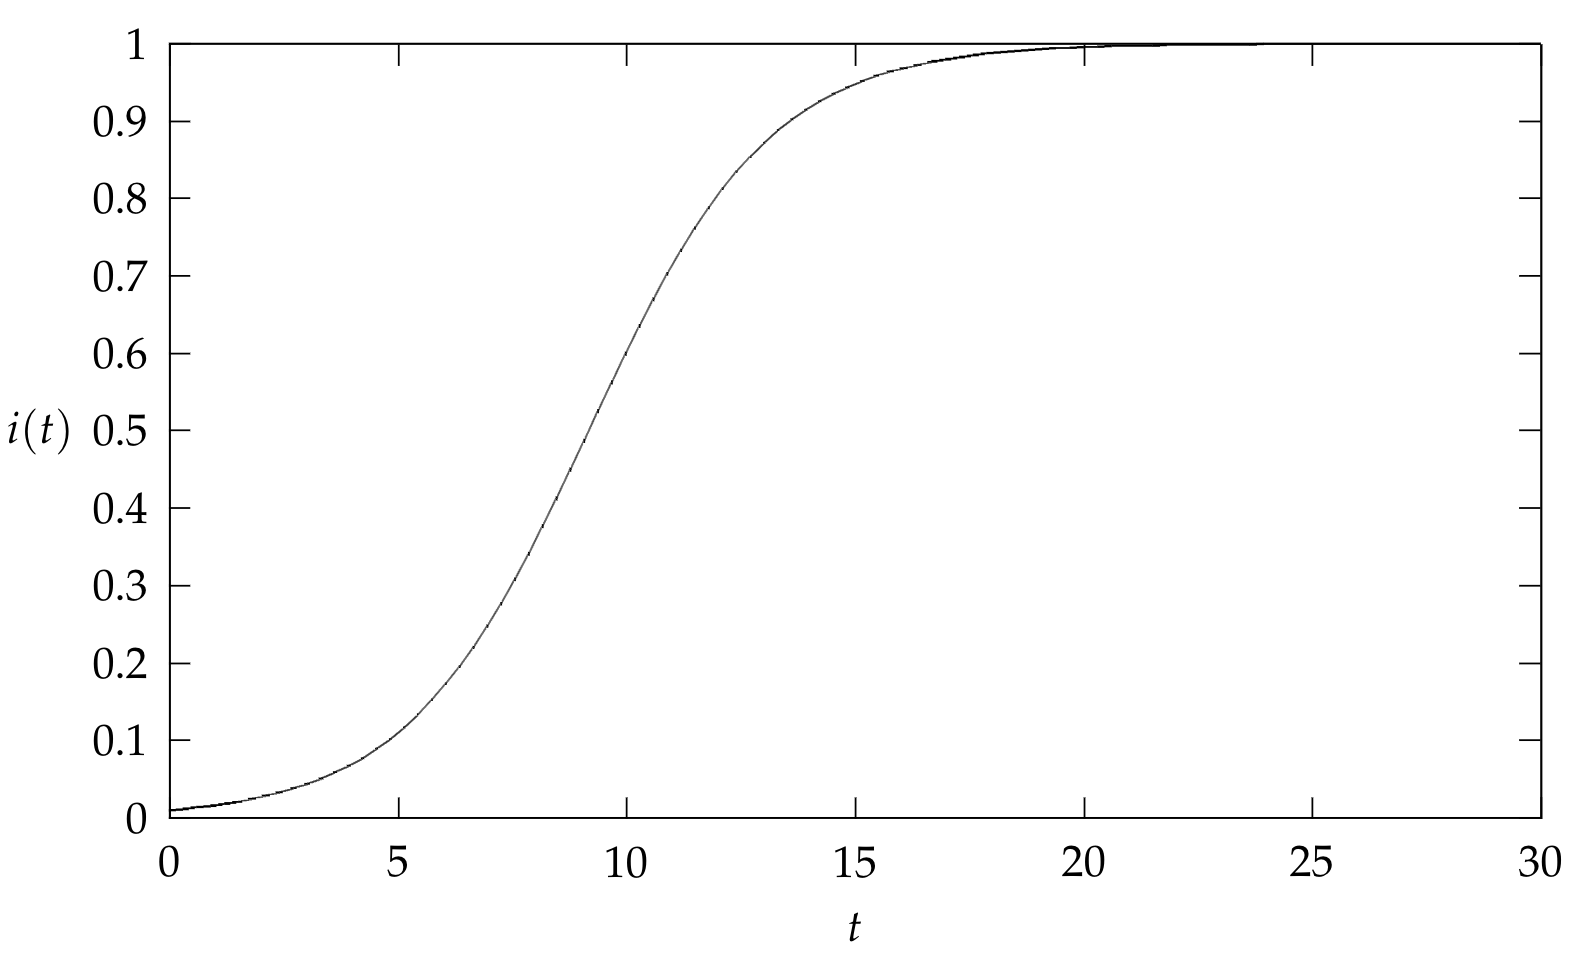
\includegraphics[height=6cm]{img/logistic_growth.png}
    \caption{Logistic growth function $i(t)$}
    \label{fig:logistic_growth}
\end{figure}

\section{SIR Model}

SIR model introduces the R state to the SI model. When, in the SI model, an individual gets infected, it remains so forever. SIR model allows infected nodes to recover from the disease after some time. In the real world, this might be because of the immune system fighting the disease. Additionally, once an individual recovers from the infection, it becomes immune to further infections. Therefore in SIR, an individual can change state only from S to I to R. In this mathematical model, we do not distinguish if the R state is obtained by immunization or death, since in both cases, an individual is removed from the potential disease hosts pool. Because of that, the model is also called susceptible-infected-removed.

Call $\gamma$ the chance of recovering from the I state. Then the ODE system for SIR model becomes:
\begin{equation}
\begin{split}
\frac{ds}{dt} &= -\beta i s \\
\frac{di}{dt} &= i \beta s - \gamma i \\
\frac{dr}{dt} &= \gamma i
\end{split}
\end{equation}

To see how this model behaves with some concrete values, consider the COVID-19 epidemic with the following assumptions: three individuals were initially infected at $t_0$, the total human population is 7.8b people, and no individual was immune to the disease at $t_0$. Hence,
\begin{align*}
I(0) &= 3 \\
S(0) &= 7.8 * 10^9 \\
R(0) &= 0
\end{align*}

We assume that each infected individual, on average, makes a possibly infecting contact once in two days (assuming homogeneous mixing across the whole globe), and the infection duration is five days: 

\begin{align*}
\beta &= \frac{1}{2} \\
\gamma &= \frac{1}{5}
\end{align*}

The following plot (Fig. \ref{fig:covid1}) shows fractions of susceptible, infectious, recovered individuals in the whole population as a function of time.

\begin{figure}[ht]
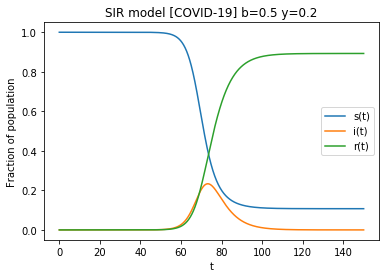
\includegraphics[width=9cm]{img/covidb12y15.png}
\centering
\caption{COVID-19 in SIR Model for $\beta=0.5$}
\label{fig:covid1}
\end{figure} 


If we decrease the number of infections to one in five days, so $\beta = 0.2$, then there is no epidemic (see Fig. \ref{fig:covid3}).

\begin{figure}[ht]
    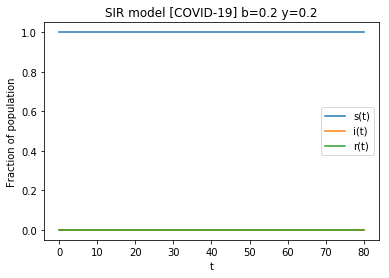
\includegraphics[width=9cm]{img/covidb15y15.png}
    \centering
    \caption{COVID-19 in SIR Model for $\beta=0.2$}
    \label{fig:covid3}
\end{figure} 

The rate of new infections $\frac{di}{dt}$ determines if an epidemic will happen; if it is positive, then there will be an epidemic, and if it is negative, individuals will recover faster than the spread of infection, so there will be no epidemic.

We can calculate the value of $\frac{di}{dt}$ at $t_0$ and check if the value is negative or positive; the negative value means the decrease of infections from the beginning, so we can be sure that eventually there will be no infections.

The condition determining if an epidemic will happen or not,is thus
\begin{equation}
i \beta s_0 - \gamma i > 0
\end{equation}
Since the fraction of infections $i$ is never negative, we can omit it to get
\begin{equation}
s_0 > \frac{\gamma}{\beta}
\end{equation}
We can introduce $R_0$, the Basic Reproduction Number:
\begin{equation}
R_0 = \frac{s_0 \beta}{\gamma}
\end{equation}
which represents the number of individuals that each infected individual can infect before recovering. Thus if $R_0 = 2$ then each infected individual can infect on average two other individual before recovering, so the number of infections grows exponentially, and if $R_0 = 0.5$, then for every two individuals, only one new infection happens, and the number of infections decreases exponentially. $R_0 = 1$ is called the \textit{epidemic threshold}, where the number of new infections equals the number of recoveries, so the total number of infected individuals is always the same and equals the initial number of infected individual $I_0$. 

For example, for seasonal flu the value of $R_0$ is estimated between 0.9–2.1 \cite{coburn2009modeling}, whereas for COVID-19 it's estimated to 2.2 in early-stage (January) \cite{li2020early} and recently to 5.7 (April) \cite{readeid}.

To mitigate an epidemic, we can decrease $s_0$ and $\beta$, or increase $\gamma$. Since we have little control over the time of recovery ($\gamma$), the only way to reduce the impact of infection is to reduce the number of contacts between infected and susceptible individuals (which is why social distancing is so crucial in a fight with epidemics).


\section{SIS Model}
There are some diseases where an individual can get infected many times, e.g., the flu. Therefore there is no Recovered population. This could be because the virus is mutating, or antibodies do not persist long enough in the organism. For this kind of epidemic, the state flow is $Susceptible → Infected → $Susceptible, hence the name SIS. 
For this kind of model, we need to modify the previous equations, so that the fraction $\gamma i$ will go to the S state, instead of the R state.
\begin{equation}
\begin{split} \label{eq_sis}
\frac{ds}{dt} &= - i \beta s + \gamma i \\
\frac{di}{dt} &= i \beta s - \gamma i
\end{split}
\end{equation}


We can solve the equations by substituting $s$ in the second equation and solving a Linear Differential Equation:
\begin{equation}
\frac{di}{dt} = i * \beta * (1 - i) - \gamma * i
\end{equation}
After integrating we get:
\begin{equation}
i = (1 - \frac{\gamma}{\beta}) \frac{C}{C + e^{-(\beta - \gamma)t}}
\end{equation}
where 

\begin{equation}
C = \frac{\beta i_0}{\beta-\gamma-\beta i_0}
\end{equation}
In Fig. \ref{fig:sis_it} we can see a plot of the function $i(t)$ for constant $\gamma = 0.2$ and $\beta = 0.5$.

\begin{figure}[h!]
    \centering
    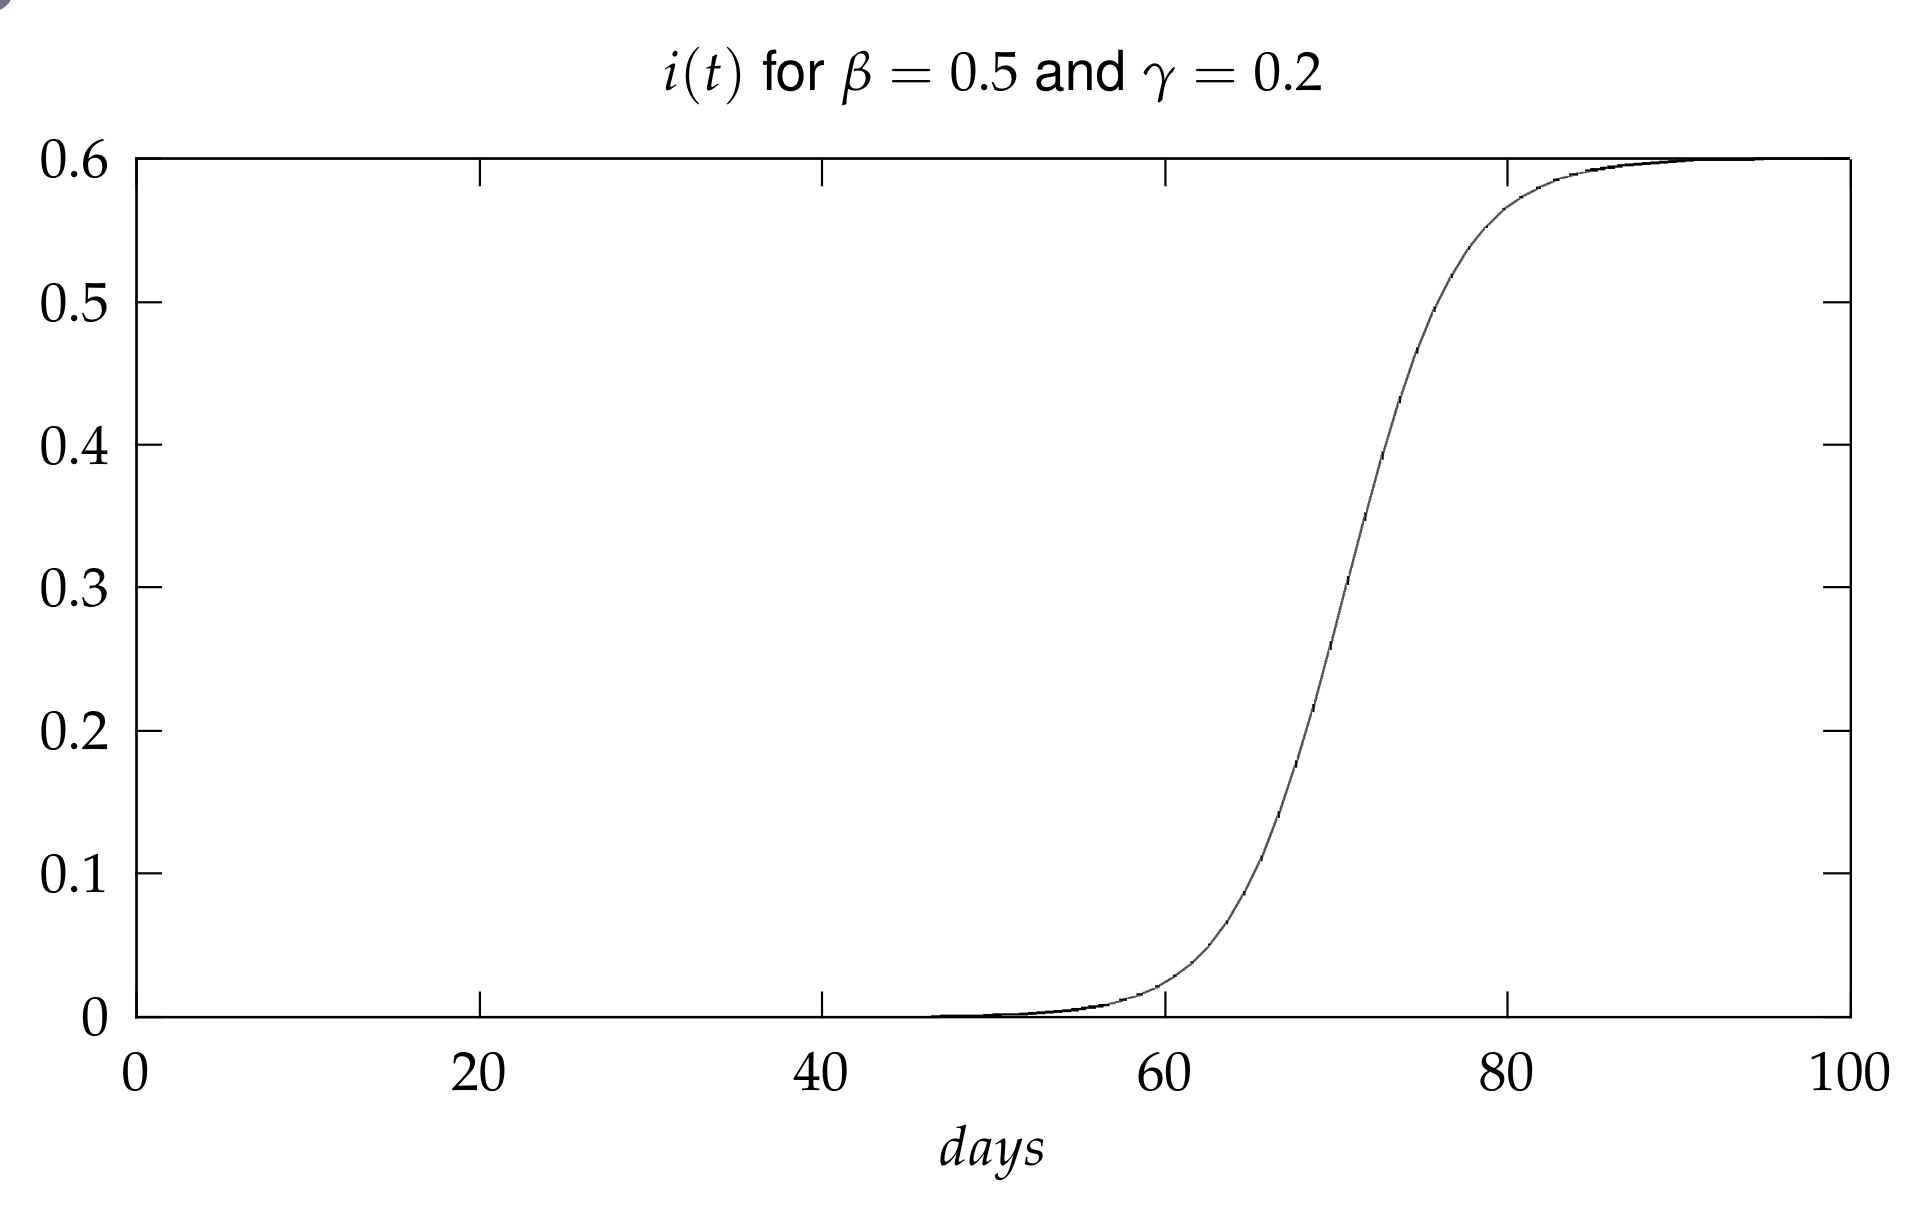
\includegraphics[height=7cm]{img/sis_it.png}
    \caption{$i(t)$ for $\beta = 0.5$ and $\gamma=0.2$}
    \label{fig:sis_it}
\end{figure}

Also, in Fig. \ref{fig:sis_ibt} we plot the function $i(t, \beta)$ for constant $\gamma = 0.2$ to see how the $\beta$ influences the results.
\begin{figure}[h!]
    \centering
    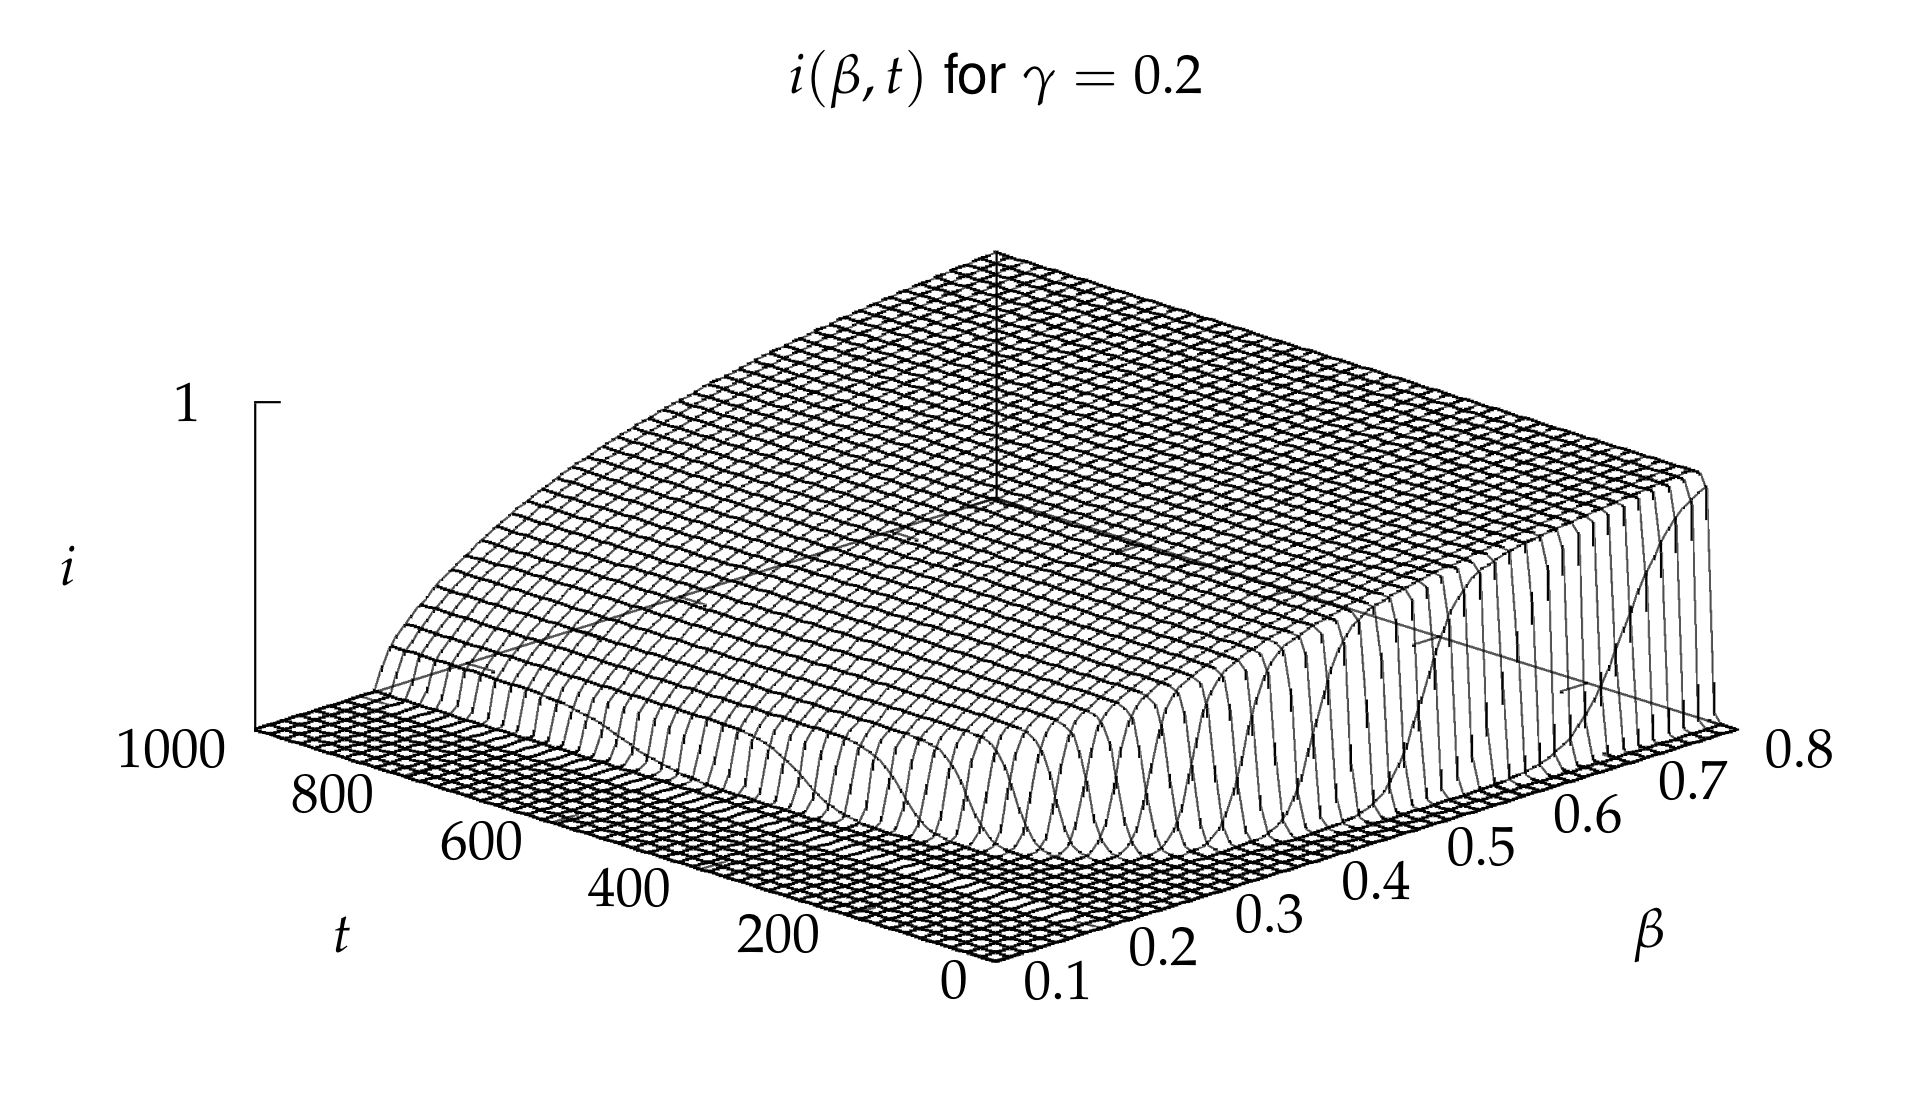
\includegraphics[width=\textwidth]{img/sis_ibt.png}
    \caption{$i(\beta,t)$ for $\gamma=0.2$}
    \label{fig:sis_ibt}
\end{figure}
As we can see, it drives the number of the infected population. If it is less than $\gamma$, the epidemic never occurs. Values greater than $\gamma$ lead to a constant fraction of the infectious population (the rate of catching the infection by the susceptible population is equal to the rate of recoveries in the infected population). The higher the $\beta$, the faster is the outbreak, and the higher the infection ratio.

\section{SIRS and SEIRS Models}
SIRS model introduces another state change, allowing recovered individuals to lose their immunity. Therefore the state flow is: $Susceptible → Infected → Recovered → Susceptible$. We can write equations for this model by simply adding one intermediate state equation to Eq. \ref{eq_sis}.
\begin{equation}
\begin{split} \label{eq_sirs}
\frac{ds}{dt} &= \delta r - i \beta s \\
\frac{di}{dt} &= i \beta s - \gamma i \\
\frac{dr}{dt} &= \gamma i - \delta r
\end{split}
\end{equation}

Another, more complex model in terms of the number of states is the SEIRS model. This model introduces an intermediary Exposed (E) state between the S and I states, where an individual is infected but does not spread infection to other people. Such modification is also easy to write by adding another intermediary state to Eq. \ref{eq_sirs}.

\begin{equation}
\begin{split}
\frac{si}{dt} &= \delta r - i \beta s \\
\frac{ei}{dt} &= i \beta s - \gamma e \\
\frac{di}{dt} &= \gamma e - \omega i \\
\frac{dr}{dt} &= \omega i - \delta r
\end{split}
\end{equation}


Clearly, these models can be easily extended to an infinite number of intermediary states, more accurately reflecting reality. Unfortunately, there is no known analytical solution to such models; they have to be solved by numerical integration of differential equations.

\section{Summary}
The above outlined models hinge on the idealistic full-mixing assumption, where each individual has an equal probability of contacting anyone else. This assumption does not reflect precisely human interaction or distributed computer networks. The $\beta$  parameter reflects a chance of an individual to contact someone else and spread the infection. In our problem, the network is static, the structure of nodes is fixed; each node has a unique set of neighbors through which the disease can spread. In real life, this might be family members, friends, or coworkers. The chance of contact with the rest of the population, like the chance of meeting two people from two ends of the earth, is minimal. For this reason, we have to consider a different model of infection dissemination. 
In our model, the infection is an abstract representing trust in content. We will look at how trust graphs are built to understand how to leverage the above mechanisms for our infection spreading model.